\usetikzlibrary{arrows}
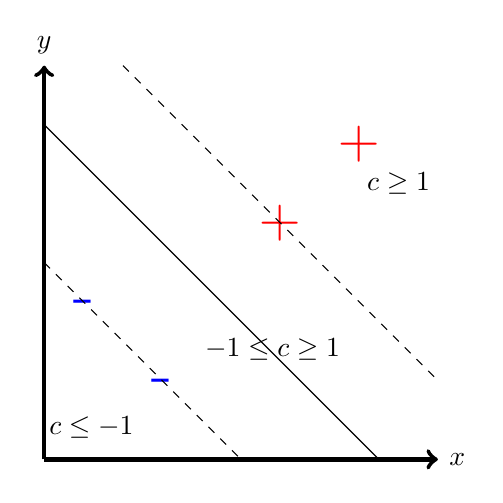
\begin{tikzpicture}


\draw[->,ultra thick] (0,0)--(5,0) node[right]{$x$};
\draw[->,ultra thick] (0,0)--(0,5) node[above]{$y$};

\node [text=blue] at (1.5,1) {\Huge -};
\node [text=blue] at (0.5,2) {\Huge -};
\node [text=red] at (3,3) {\huge +};
\node [text=red] at (4,4) {\huge +};



\draw[dashed]  (1,5)--(5,1);
\draw[dashed]  (0,2.5)--(2.5,0);
\draw(0,4.25)--(4.25,0);


\node at (4.5,3.5) {$c \geq 1$};
\node at (0.6,0.4) {$c \leq -1$};
\node at (2.9,1.4) {$ -1 \leq c \geq 1$};

\end{tikzpicture}
